\documentclass[12pt,portuguese,a4paper]{article}
\usepackage[T1]{fontenc}
\usepackage[scaled]{luximono}
\usepackage{amsmath}
\usepackage{babel}
\usepackage{graphicx}
\usepackage{epstopdf}
\DeclareGraphicsRule{.tif}{png}{.png}{`convert #1 `dirname #1`/`basename #1 .tif`.png}

\usepackage[applemac]{inputenc}



\usepackage{natbib}
\usepackage{color}
\usepackage{colortbl}
\usepackage[colorlinks,urlcolor=blue]{hyperref}
%\usepackage{url}
\usepackage{fancybox,calc}
\usepackage{alltt}
\usepackage{makeidx}
\usepackage{fancyvrb}



%%% PACKAGES
\usepackage{booktabs} % for much better looking tables
\usepackage{array} % for better arrays (eg matrices) in maths
\usepackage{paralist} % very flexible & customisable lists (eg. enumerate/itemize, etc.)
\usepackage{verbatim} % adds environment for commenting out blocks of text & for better verbatim
\usepackage{subfigure} % make it possible to include more than one captioned figure/table in a single float
% These packages are all incorporated in the memoir class to one degree or another...




%%% Para o c—digo
\usepackage{listings}
\lstloadlanguages{Python,C,Java,Prolog,Lisp}

\lstset{backgroundcolor=\color{yellow},language=Python,captionpos=b,showstringspaces=false,basicstyle=\ttfamily,commentstyle=\color{blue},tabsize=2,breaklines=true}

%% E mais umas coisas
\usepackage{multirow} % para tabelas
\usepackage{pifont} % para fontes e s’mbolos
\usepackage{marvosym} % para s’mbolos
\usepackage{lettrine} % para iniciar o texto de modo especial
\usepackage{epigraph} % para bocas cŽlebres...
%\usepackage{chicago}


\renewcommand\lstlistingname{Listagem}

\DeclareUrlCommand\email{\urlstyle{rm}}
% 
    % \renewcommand\UrlLeft{e-amail:\ }%
     %\renewcommand\UrlRight{}}

% cores 
\definecolor{cinza}{rgb}{0.7,0.7,0.7}

% Comecemos!!!

\title{\Large{\textbf{Como fazer?}}}

\author{\textbf{Ernesto J. F. Costa} \\ \email{ernesto@dei.uc.pt}\\Departamento de Engenharia Inform‡tica \\ Universidade de Coimbra}


\date{\today} 





%%% BEGIN DOCUMENT
\begin{document}

\maketitle

\begin{abstract}
Este pequeno texto pretende exemplificar o modelo de documento que devem entregar. Identifica as suas sec\c c›es principais. TambŽm serve para verem como se podem fazer algumas certas coisas em \LaTeX{}. O vosso documento deve ter tamanho m‡ximo de 15 p‡ginas, podendo este limite apenas ser ultrapassado se, justificadamente, for necess‡rio incluir tabelas e/ou imagens. A entrega deve ser feita atŽ ao final do ms de Maio. Acompanha o texto referido, o programa em suporte magnŽtico, com um pequeno manual do utilizador. Todo o material pode ser enviado por correio electr—nico. No entanto, o texto principal tem que ser entregue em papel. Pode ser deixado no meu cacifo de correio.
\end{abstract}

\epigraph{Ser ou n‹o ser. Eis a quest‹o!}{Shakespeare}

\section{Introdu\c c‹o}

\lettrine{E}{screver um artigo}, um livro, uma tese, e por a’ fora, tem regras. Uma consulta na internet pelas palavras \textit{write paper} far‡ aparecer v‡rios documentos (ver por exemplo um em \url{http://www.ruf.rice.edu/~bioslabs/tools/report/reportform.html}). TambŽm exitem v‡rios livros sobre o assunto (ver  \cite{davis1997}, \cite{deal2010}, \cite{murray2007}). O que se segue s‹o indica\c c›es genŽricas sobre o que deve constar em cada sec\c c‹o. J‡ agora. Quem quiser iniciar-se ao \LaTeX{} pode ir a \url{http://www.tug.org/} onde encontrar‡ toda a informa‹o necess‡ria \footnote{Para os pregui\c cosos: vou colocar alguns textos introdut—rios em pdf na p‡gina da cadeira}. Quem quiser saber mais (muito mais \ldots), consulte a b’blia sobre o assunto \cite{mg2004}. Note que \textcolor{red}{\textbf{n‹o}} Ž obrigado a fazer em \LaTeX{}, mas apenas aconselhado.\\



\textit{Aqui deve ser descrito qual o tema, a sua import‰ncia, os objectivos do trabalho e o modo como o texto est‡ organizado.}


\section{Problema} 

\lettrine[lines=2,lraise=0.2]{S}{— para exemplificar} outro modo de come\c car uma sec\c c‹o. Claro que n‹o Ž obrigado a fazer as coisas deste modo. Como hoje Ž sexta, faz muito calor  e l‡fora o dia est‡ bonito, deu para masoquisticamente me castigar. H‡ coisas piores eu sei. Mas h‡ coisas em rela\c c‹o ˆs quais n‹o consigo resistir. ƒ isso e estar a escrever patetices s— para ter texto suficiente para o efeito que pretendo exemplificar sair real\c cado. Ou n‹o \ldots\\\\

\textit{Descrever o problema que vai ser tratado.}

\section{Estado da Arte}

\textit{Acrescentar  aqui uma breve referncia aos diferentes modos como o assunto tem sido tratado. Repito: breve! }\\


{\textbf{\color{red} As duas  sec\c c›es Problema e Estado da Arte podem eventualmente ser fundidas numa s—.}}

\section{Metodologia}

\textit{
Qual a abordagem metodol—gica seguida. Porque (e como)  foram escolhidos os testes estat’sticos? Que experincias foram feitas? Qual a parametriza\c c‹o?
}\\

\subsection{Tabelas}

Isto das tabelas em \LaTeX{} pode ser um bom quebra-cabe\c cas \ldots J‡ existem algumas aplica›es que facilitam a vida, mas conte com algum tempo para fazer uma tabela complexa {\Large{\Frowny}}. \\ Veja o exemplo de tabela \ref{tab:ola}.

\begin{table}[htdp]
\begin{center}
\begin{tabular}{|c|cc|cc|cc|cc|} \hline
\raisebox{-1.5ex}[0cm][0cm]{Tipo} & \multicolumn{8}{c|}{Fun\c c‹o}\\ \cline{2-9}
& \multicolumn{2}{c|}{$F_{1}$} & \multicolumn{2}{c|}{$F_{2}$} &\multicolumn{2}{c|}{$F_{3}$} & \multicolumn{2}{c|}{$F_{4}$} \\ \hline 
Pop & 10  & 100  & 10  & 100 & 10  & 100 & 10  & 100 \\ \hline 
GA &  2 & 3 & 4 & 5 & 6 & 7 & 8 & 9 \\ \hline
EE &  2 & 3 & 4 & 5 & 6 & 7 & 8 & 9 \\ \hline
GP &  2 & 3 & 4 & 5 & 6 & 7 & 8 & 9 \\ \hline
\end{tabular}
\end{center}
\caption{Uma tabela}
\label{tab:ola}
\end{table}

Outro modo de obter o mesmo resultado, agora usando o comando \texttt{multirow} Ž ilustrado na tabela \ref{tab:ola2}. E j‡ agora vamos p™r {\textcolor{green} {cor}} nesta coisa.

\begin{table}[htdp]
\begin{center}
\begin{tabular}{|c|cc|cc|cc|cc|} \hline
 \multirow{2}{*}{Tipo} & \multicolumn{8}{> {\columncolor{red}}c|}{Fun\c c‹o}\\ \cline{2-9}
& \multicolumn{2}{c|}{$F_{1}$} & \multicolumn{2}{c|}{$F_{2}$} &\multicolumn{2}{c|}{$F_{3}$} & \multicolumn{2}{c|}{$F_{4}$} \\ \hline 
\rowcolor{cinza} Pop & 10  & 100  & 10  & 100 & 10  & 100 & 10  & 100 \\ \hline 
GA &  2 & 3 & 4 & 5 & 6 & 7 & 8 & 9 \\ \hline
EE &  2 & 3 & 4 & 5 & 6 & 7 & 8 & 9 \\ \hline
GP &  2 & 3 & 4 & 5 & \multicolumn{1} {>{\columncolor{blue}} c} {\textcolor{white}{6} }& 7 & 8 & 9 \\ \hline
\end{tabular}
\end{center}
\caption{A mesma  tabela}
\label{tab:ola2}
\end{table}

% for\c car uma nova p‡gina 

\pagebreak[4]

\subsection{Imagens}

Precisa de uma figura?? N‹o se admire se a figura \ref{fig:dist1} n‹o aparecer exactamente onde a colocou no texto. Tabelas e imagens flutuam no texto havendo no entanto algumas possibilidades de controlar a sua coloca‹o. Ës vezes basta apenas alterar a sua dimens‹o usando o par‰metro \textit{scale}. Se olhar para o texto fonte ver‡ outro modo de controlar o posicionamento.

\begin{figure}[!htbp] % h= here, t= top; b=bottom, != onde for poss’vel
\begin{center}
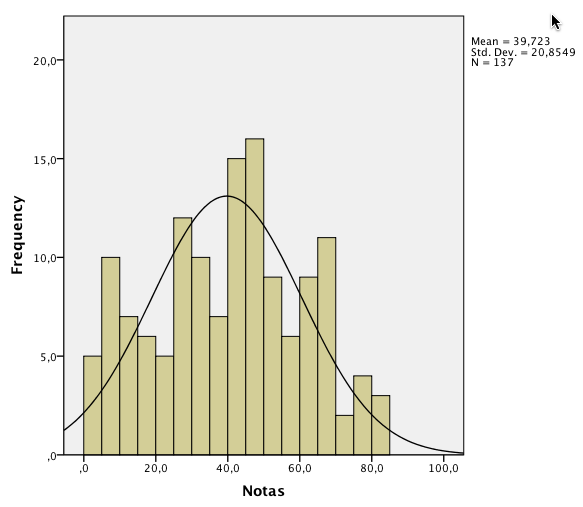
\includegraphics[scale=0.5]{imagens/dist.png}
\caption{{\bf A minha distribui\c c‹o}}
\label{fig:dist1}
\end{center}
\end{figure}

\section{Resultados e Discuss‹o}

\textit{
Aqui aparece um resumo das experincias realizadas e uma discuss‹o do seu significado.
}

\section{Conclus‹o}

\textit{
Terminar Ž terminar. Retoma-se o objectivo, as conclus›es principais, e avan\c ca-se com a indica\c c‹o do que ficou por fazer e do eventual trabalho futuro \Large{ \Smiley}.
}

\appendix

\section{O que tiver que ser}

\textit{
O que n‹o tem sentido colocar no corpo principal do programa mas pode ser importante para a compreens‹o.
}

\section{E mais outra coisa}

Quem usar um computador Apple Macintosh encontra em \url{http://www.tug.org/mactex/} o melhor produto para \LaTeX{}. Gr‡tis! Para outras plataformas (Windows, Linux) usar o TeXLive. Informa›es em \url{http://www.tug.org/texlive/}.

\bibliographystyle{plain}
% O nome do ficheiro com as referncia bibliogr‡ficas deve ter a extens‹o .nib!
\bibliography{tp}

\end{document}